\documentclass[9pt,twocolumn,twoside,lineno]{pnas-new}
\templatetype{pnasresearcharticle}

%\usepackage[margin=.8in]{geometry}
%\usepackage{graphicx}
%\usepackage{amsmath}
%\usepackage{amssymb}
%\usepackage{titlesec}
%\usepackage[numbers]{natbib}
%\usepackage{sidecap, caption}
\usepackage{subcaption}
\usepackage[figuresleft]{rotating}
\usepackage{fixme}
\newcommand{\at}{\makeatletter @\makeatother}
%\titlespacing*{\section}
%{0pt}{2ex}{0ex}
%\titlespacing*{\subsection}
%{0pt}{2ex}{0ex}
%\titlespacing*{\subsubsection}
%{0pt}{2ex}{0ex}
%\font\myfont=cmr12 at 16pt

\graphicspath{{../plots/}}

\title{The Wisdom and Persuadability of Threads}

% Use letters for affiliations, numbers to show equal authorship (if applicable) and to indicate the corresponding author
\author[a,1]{Robin Engelhardt}
\author[a]{Jacob Stærk-Østergaard}
\author[a]{Vincent F. Hendricks}
\affil[a]{Center for Information and Bubble Studies, Department of Communication, University of Copenhagen, Karen Blixens Plads 8, DK-2300 Copenhagen S.}


% Please give the surname of the lead author for the running footer
\leadauthor{Engelhardt} 

% Please add here a significance statement to explain the relevance of your work
\significancestatement{Online discussion threads are important means for individual decision-making as well as for aggregating collective judgments. Empirical and theoretical investigations of this `wisdom of crowds' are currently ambivalent about the role played by social information. While some findings suggest that social information undermines crowd accuracy due to correlated judgment errors, others show that accuracy improves. We demonstrate that, for difficult tasks, seeing preceding estimates aids individual decision-making as well as collective accuracy in pristine threads, but not in manipulated threads where participants only see the most extreme estimates. By assigning a persuadability score to each estimate, we additionally show that persuadability depends on task difficulty as well as on the amount of social information received.
}

% Please include corresponding author, author contribution and author declaration information
\authorcontributions{R. E. designed the experiment and analyzed the data and contributed as lead author, J. S-Ø. analyzed the data and contributed as co-author, V.F.H. contributed as the co-author and as the project manager.}
\authordeclaration{The authors declare no conflict of interest.}
%\correspondingauthor{\textsuperscript{1}ORCID: 0000-0002-7162-0990}
\correspondingauthor{\textsuperscript{1}To whom correspondence should be addressed. E-mail: robin\at hum.ku.dk}


% Keywords are not mandatory, but authors are strongly encouraged to provide them. If provided, please include two to five keywords, separated by the pipe symbol, e.g:
\keywords{collective intelligence $|$ magnitude estimation $|$ decision-making $|$ discussion threads $|$  social networks} 


\begin{abstract}
Social decision-making is increasingly relying on digitized aggregates of people’s opinions and judgments. These aggregates are frequently maintained as threads, i.e. as sequences of posts on a website. While it has been shown that knowledge of thread aggregates can distort individual decision-making, it is unknown how seeing preceding posts in a thread may influence collective accuracy, i.e. the wisdom of threads, as well as individual persuadability. We investigate experimentally the accuracy of threads in which people make magnitude estimations of varying difficulty and varying degrees of social information in the form of visible previous estimates. We find a significant increase in collective accuracy for high difficulties and high levels social information in pristine threads, while collective accuracy declines quickly under the same conditions in manipulated threads. Using gaussian mixture models we assign a persuadability score to each participant, and show that persuadability generally increases with task difficulty and with the amount of social information. In the case of strong manipulation, we may see a split between a minority of persuadables and a majority of skeptics.
\end{abstract}

\dates{This manuscript was compiled on \today}
\doi{\url{www.pnas.org/cgi/doi/10.1073/pnas.XXXXXXXXXX}}

\begin{document}

\maketitle
\thispagestyle{firststyle}
\ifthenelse{\boolean{shortarticle}}{\ifthenelse{\boolean{singlecolumn}}{\abscontentformatted}{\abscontent}}{}

\dropcap{S}ocial information in the form of opinions and judgments by other people is sampled sequentially. We read the news, hear rumors, listen to debates on TV, and flip through comments on social media platforms and blogs. These activities inform us and influence our decisions, but researchers still debate the conditions under which these types of social information help us make better decisions \cite{woolley2010evidence, gurccay2015power, becker2017network, jayles2017social}, lead us astray \cite{caplan2011myth, lorenz2011social, minson2012cost, king2011true, le2018endogenous}, or just make us confused at a higher level \cite{salganik2006experimental, salganik2009web}.

Collective estimates of a diverse group of people can outperform the majority of its members because any random confusion at the individual level is likely to average out and let the most accurate estimate prevail \cite{galton1907vox, muth1961rational, surowiecki2005wisdom, hong2008some}. Then again, confusion is not always randomly scattered around the truth. Systematic biases in individual perception may create measurable disruptions in the wisdom of crowds \cite{izard2008calibrating, nash2014curious, kao2018counteracting}. Social information can add to those biases and create cascades, echo chambers, bandwagoning and herd behavior \cite{anderson1997information, bikhchandani1992theory, bakshy2015exposure, banerjee1992simple}. Partially sampled social information may lead to rich-get-richer dynamics \cite{barabasi1999emergence} and to belief misattributions, which uphold harmful social practices despite being rejected by a majority of people \cite{katz1931students, darley1968bystander, ross1977false, noelle1974spiral, lee2019homophily}. Social information may also have been intentionally filtered or manipulated in various ways, for instance through group pressure \cite{asch1951effects}, algorithmic filtering \cite{pariser2011filter}, false cues \cite{salganik2006experimental, muchnik2013social, hanson1996hits}, or simply by plain misinformation \cite{hendricks2018reality}, often with highly detrimental consequences for our economy and our health.

Observational data of decision-making processes is acutely sensitive to the social context in which people find themselves. Thus, researchers find it difficult to separate observational data into its social and individual components. How may we know how much weight an individual puts on her own ‘independent’ estimate relative to the weight put on the estimates by others? Randomized experimental studies have attempted to solve this problem by first letting participants make a magnitude estimate of an object without social information (\textit{ex ante}), and subsequently ask them to revise their estimate after having received information about other people’s estimates of that object (\textit{ex post}) \cite{becker2017network, jayles2017social, lorenz2011social, sniezek1995cueing, mavrodiev2013quantifying}. This double elicitation paradigm presumes that people change their mind because of the social information they have received. Other studies, however, have shown that people routinely can change their mind all by themselves, and that it may be more correct to assume an `inner crowd' in the sense that people sample randomly from a probability distribution in their own mind \cite{vul2008measuring, herzog2009wisdom, herzog2014harnessing}. Such a psychological mechanism - and maybe others such as hedging strategies due to anticipated regrets \cite{bell1982regret}, and/or disappointments \cite{loomes1986disappointment} - make it difficult to differentiate between `inner' samples and `outer' influences, and it may therefore be desirable to develop an alternative framework that is able infer the extend of individual bias and social influence from a single estimation task.

We propose to use probabilistic gaussian mixture models (GMMs) since they have properties that are highly valuable in the context of crowd aggregation research. First, GMMs are comprised of several Gaussians which fit well to the highly right-skewed and long-tailed distributions emerging from free response elicitations. Second, GMMs associate a measure to each data point, describing the influence of social information on that particular participant. This measure aids us in associating participants with sub-populations in the data related to how people act under available social information, without using any prior knowledge of these sub-populations. FINALLY, as a statistical model, GMMs provide confidence bounds to the estimates, which further adds a measure of model certainty.

We also propose the experimental mechanism of dot-guessing games \cite{horton2010dot}, where participants guess the number of dots in an image. While dot estimations have been used previously in numerosity experiments \cite{minturn1951effect, indow1977scaling, krueger1982single} they have only recently been proposed as useful ‘model organisms’ for crowd aggregation research \cite{horton2010dot, ugander2015wisdom} due to their advantages in terms of cultural neutrality, resistance to expertise and/or prior knowledge, and their qualities as captchas \cite{von2008recaptcha}. In addition, dot estimation tasks are easy to implement and easy to understand. Most importantly, they have an objective solution and are tunable, allowing for nearly-continuous difficulty levels and performance measures.

\section*{Experimental Design}
We collected a total of 11,748 estimates from 6,196 unique participants on Amazon Mechanical Turk. 5,990 estimates were collected from participants placed in 12 different threads where they successively estimated the number of dots, $d \in \{55,148,403,1097\}$, in an image, while seeing $v \in \{1,3,9\}$ \textit{preceding} estimates (historical threads). Another 3,934 estimates were collected from participants who were placed in 12 other threads and shown the same images while seeing the $v \in \{1,3,9\}$ \textit{highest} estimates made so far (manipulated threads). Finally, 1.824 estimates were collected from participants who were shown the same images, but with $v=0$, corresponding to control conditions for each $d$ containing no social information. 

We interpret the number of dots, $d$, as the \textit{task difficulty}, while the number of visible previous estimates, $v$, is interpreted as the \textit{degree of social information}. Participants were placed randomly in one of the 28 threads ($2 \times 3 \times 4$ + 4 controls)  and made their estimate one after another. In order to keep the estimates in a somewhat realistic range, participants could not submit numbers below 10 and above 1.000.000. No participant who had seen a certain image would be able to participate in another thread containing the same image again. In addition to a participation fee and a variable waiting fee, all participants in all threads received a bonus of \$1 if their estimate was within 10\% of the true value. See the Materials and Methods section and the Appendix for additional information about the experimental design.

\section*{Methods}
Free response elecitation of absolute values is known to create right-skewed distributions with long tails, which inflate the means. While it is still debated which measure is best suited to aggregate such data \cite{kao2018counteracting}, we follow the lead of Galton \cite{galton1907vox} and focus on the median as it is easy to interpret, robust against outliers, and best expresses the opinion of the crowd in the sense that the majority deems every other estimate as too high or too low. For the statistical analysis of thread aggregates, we therefore compare the log-ratio of thread medians, $y_{dv}=\log(M_{(d,v)}/d)$, using a linear normal model to quantify differences between threads in terms of $\log(d)$ and $v$, the latter as a categorical variable. The effects of social information on individual descision-making are analysed using probabilistic gaussian mixture models on the log-ratio of individual estimates with the geometric mean of the social information as the explanatory variable. 

In each thread, datapoints are divided into states with corresponding independent gaussian components. 

\textcolor{red}{schematic illustration here}. 

Let $Y$ denote the observation and $X\in\{1,2,\dots,k\}$ denote the state. Then the conditional variable $Y|X$ is gaussian with parameters depending on the state $X$. As an example, let $X=\{1,2,3\}$, i.e. we assume a model with $k=3$ possible states. Then $Y|X=i \sim \mathcal{N}(\mu_i,\sigma_i^2)$ for $i=1,2,3$. Using notation $\delta = (\delta_1,\dots,\delta_k)$ as the estimated weight of each state, with $\delta_i >0$ and $\sum_{i=1}^k\delta_i = 1$, then the unconditional distribution of $Y$ becomes $P(Y) = \sum_{i=1}^k \delta_i P(Y|X=i)$, that is a weighted sum of gaussian probabilities, hence the name *gaussian mixture model* (GMM). This model structure can compensate for the heavy tails by adapting the different states to the more/less extreme observations.  To keep things tractable we set the number of states to $k\in\{2,3,4\}$ and then pick the number of states with the lowest BIC, conditional on convergence in the fitting routine (see section `Information criteria' in Materials and Methods). The model is fitted by the expectation-maximization (EM) algorithm using the `depmixS4` package in `R` (ref?). The $\mu_i$ parameter is extended, as in standard a linear regression model, with linear coefficients $\beta_{ij}, i=1,\dots,k, \quad j=1,\dots,p$, that can account for the social information present (see details of model specifications in Materials and Methods, section `Analysis of social information').

%In order to assess the relative strength and weakness of our single elicitation paradigm, we use our model framework with ex post data from \citet{jayles2017social}, in which a double elicitation paradigm was used. For improved comparison, we choose threads with 1 and 3 views and with 1097 and 403 dots, as those tasks are closer to the difficulty level used by \citet{jayles2017social} (see Appendix). Overall, we find a similar distribution of states (?) and similar average levels of social influence (\textcolor{red}{skal tjekkes}), but an orthogonal (or complementary? or different?) categorization of participants according to how they react to the social information (see Appendix, section Z). (det her skal formuleres bedre...)


\begin{figure*}[!h]
\centering
	\begin{subfigure}[t]{.46\linewidth}
		\centering
		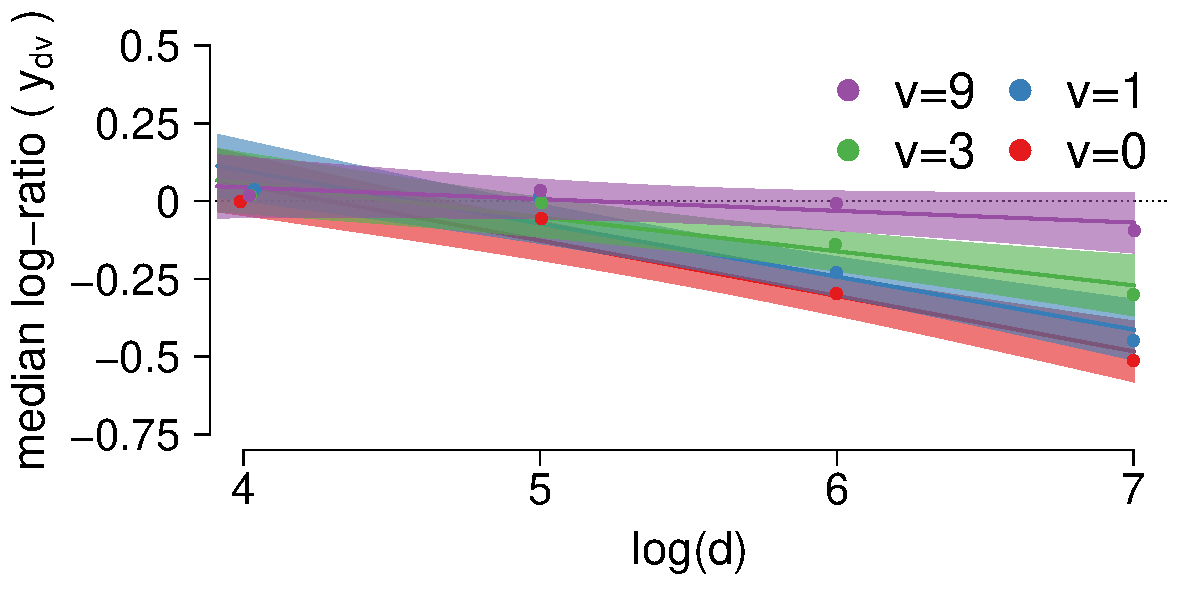
\includegraphics[width=1\linewidth]{med_confidence_h.pdf}	
		\caption{\footnotesize Historical threads.}
		\label{fig: median confidence bounds - historic}
	\end{subfigure}
	\begin{subfigure}[t]{.46\linewidth}
		\centering
		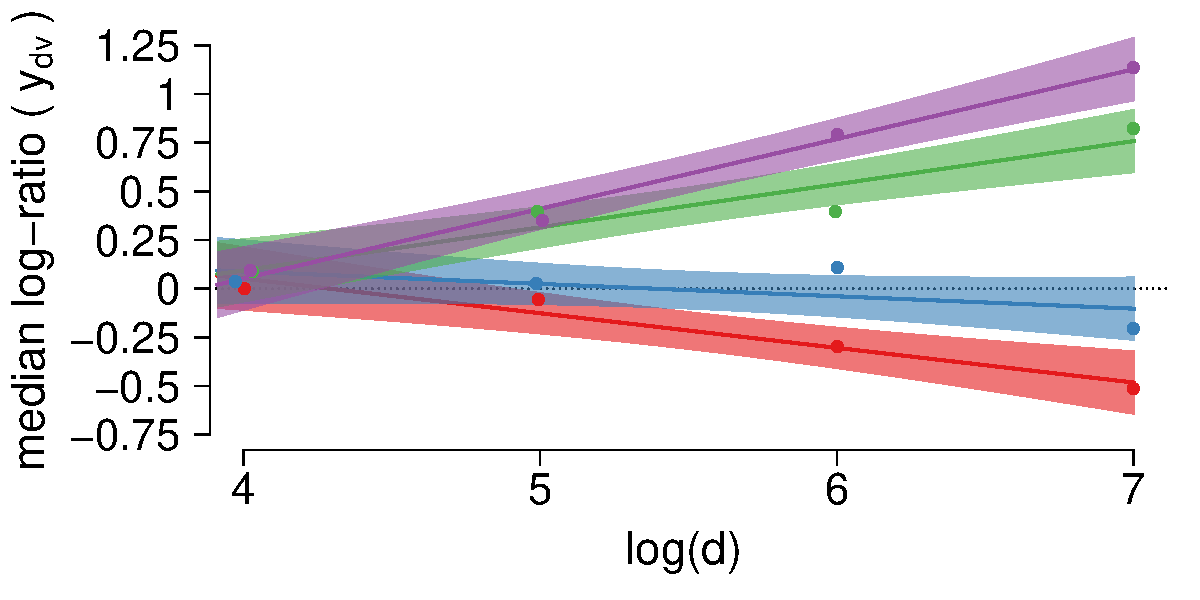
\includegraphics[width=1\linewidth]{med_confidence_m.pdf}		
		\caption{\footnotesize Manipulated threads.}
		\label{fig: median confidence bounds - manipulated}
	\end{subfigure}
	\caption{\textbf{Thread accuracy}. Relationship between median log-ratio $y_{dv}$ and $\log(d)$ with 95\% confidence bounds (shaded areas). Colors represent the number of visible estimates, $v$. There is a clear relation between $d$ and $v$ in both thread types showing that social information plays a dual role in difficult tasks: When $v$ is large, unmanipulated social information \textbf{(a)} counteracts underestimation bias and improves thread accuracy. When the social information is manipulated \textbf{(b)}, however, a strong overestimation bias emerges for large $v$. The red lines corresponding to the control groups with $v=0$ are identical in both plots.}
	\label{fig: median confidence bounds}
\end{figure*}

\section*{Results}
In accordance with previous findings, participants do well in tasks without social information, especially when estimating small numbers. For higher difficulties estimates vary widely and biases become substantial \cite{indow1977scaling, izard2008calibrating, krueger1982single, krueger1984perceived, kao2018counteracting}. The median tends to underestimate the true value and the mean tends to overestimate the true value. Summary statistics of all 28 treatments can be inspected graphically and in table format in the Appendix, section X and Y.

%While Galton only found a 0.8\% difference between the median estimate and the true weight of a slaughtered ox \cite{galton1907vox}, we find the median estimate of our ox to be less than half the true weight of the ox, as can be seen in the control condition $v=0$ in the top left panel of fig. \ref{fig:1}.

%\begin{figure*}[!ht]
%\centering
%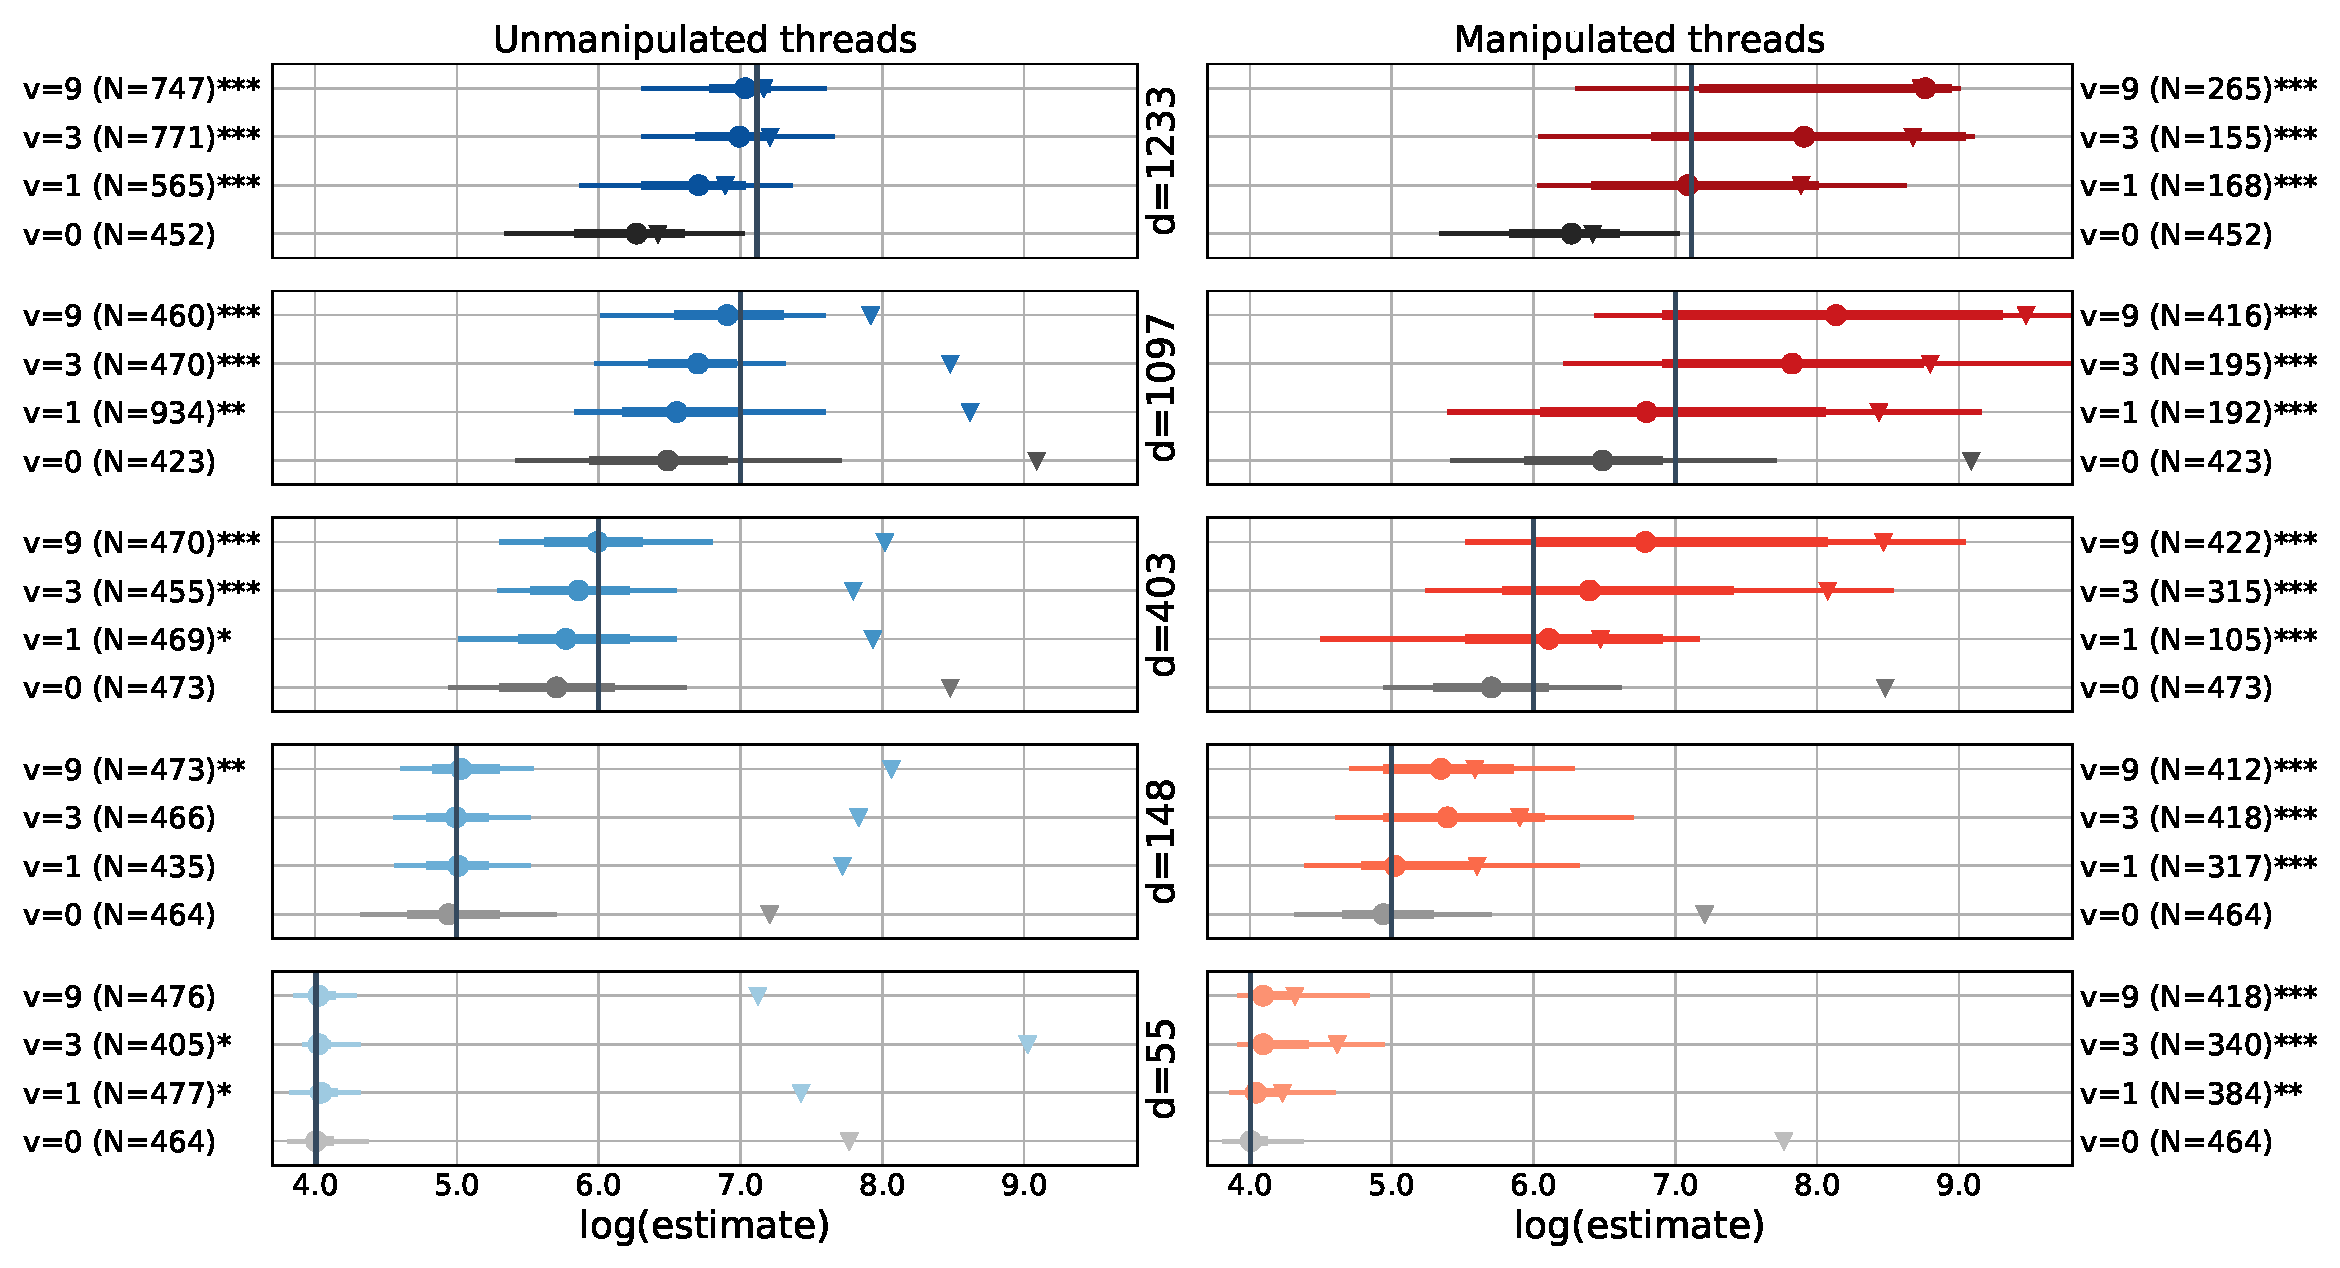
\includegraphics[width=1\linewidth]{../plots/fig1max.pdf}
%\caption{\small \textbf{Left:} Summary statistics of $d \times v$ treatments with a total of 10.348 magnitude estimates of either the number of dots in an image, $d \in \{55,148,403,1097\}$, or the weight of an ox, $d \in \{1233\}$, while participants are able to see $v \in \{0,1,3,9\}$ preceding estimates. Greys are the control treatments with $v=0$. Estimates are log-transformed. Large circles indicate medians, triangles indicate arithmetic means, thick lines show interquartile ranges, thin lines show interdecile ranges, vertical black lines show the true value, and stars indicate significance levels compared to the control treatment (two-sided Wilcoxon-Mann-Whitney test). No outliers were removed, making the arithmetic means strongly right skewed. \textbf{Right:} Summary statistics of $d \times v$ treatments with a total of 4.522 additional magnitude estimates, where participants do not see the preceding estimates but the $v \in \{1,3,9\}$ \textit{highest} estimates made so far. The controls, $v=0$, are the same as on the left hand side.}\label{fig:1}
%\end{figure*}

%The inclusion of social information, however, changes collective performance profoundly. As soon as participants can see preceding estimates in the unmanipulated threads, median accuracy improves substantially in the difficult tasks, see the horizontal boxplots on the left hand side of figure \ref{fig:1}. The interquartile and interdecile ranges show large variations, however, which tend to increase with $d$ (keeping $v$ fixed) and decrease with $v$ (keeping $d$ fixed). 

%The right hand side of figure \ref{fig:1} shows the equivalent results for the manipulated threads. Participants quickly start to overestimate, even with $v=1$. For higher $d$ and $v$, estimates inflate ever more. 

%In fact, we were able to create threads in which a majority of participants estimated the ox ($d=1233$) to weigth more than 6000 kilo. Clearly, in the begining of a thread, only a few of the $v$ visible estimates presented as social information may be high numbers. But at later times, the social information consists of even more high numbers, maybe making it more difficult to resist their influence. At a certain point, however, all of the visible estimates may become so improbably high, that some participants may suspect foul play and start to ignore them (see section `Effects of social information').

\subsection*{Analysis of thread performance}
The relationship between the observed median ratio $y_{dv}$ and the number of dots $d$ were found to be optimal, according to quantile-quantile plots (see Appendix), when modeling $y_{dv}$ against $\log{d}$. We thus quantify the overall differences between threads in terms of the log-ratio of their medians, $y_{dv}=\log(M_{(d,v)}/d)$, as a function of $\log(d)$ and $v$. Historical and manipulated threads are modeled separately.

Figure \ref{fig: median confidence bounds - historic} shows that the collective performance of historical threads declines significantly with increasing task difficulty (higher $d$), but improves when the social information is substantial (high $v$). In contrast to \cite{lorenz2011social, king2011true, minson2012cost} and in concert with \cite{gurccay2015power, becker2017network, jayles2017social, farrell2011social} these findings support the claim that crowds indeed may become wise under (pristine) social influence. It should be noted, however, that the overlapping confidence intervals reveal where thread performances are comparable. Thus, the negative effects of task difficulty and the positive effects of social information are only discernible in situations where people have hard problems to solve and at the same time have plenty of social information available. In fact, the median estimate of all historical threads with $v=9$ is `wise' in the sense of being statistically indistinguishable from the true value.

In manipulated threads, Fig.\ref{fig: median confidence bounds - manipulated}, the manipulation gives a large positive bias for $v=3,9$ which increases with $d$, implying that when a task becomes more demanding, the amount of (filtered) social information has a highly detrimental impact on thread performance. For $v=1$ there is still a small negative trend, meaning that the manipulation is not very effective. This resonates well with findings in \cite{jayles2017social}, who show that providing a moderate amount of incorrect information can counterbalance underestimation bias and improve collective performance. We add to this that as a task becomes demanding, the amount of filtered (or manipulated) social information has a significant negative impact on thread performance. %Large amounts of pristine and unmanipulated social information, however, has a noticeable positive impact on thread performance.

\subsection*{Social Influences on Decision-making} 
A GMM (see eq. \ref{eq: weighted Gaussian parameters} in Materials and Methods) was fitted to all threads using the geometric mean of visible estimates as a proxy for the available social information. For each model, the standardized residuals (eq. \ref{eq: GMM residuals} in Materials and Methods) were evaluated visually using quantile-quantile plots against a standard normal $\mathcal{N}(0,1)$. These plots (see Figure \ref{fig: qq plots AMT data} in the Appendix), reveal that models using $k=2,3,4$ states fitted the data quite well, with only a few models displaying a less adequate fit. 
%This could indicate that either a larger $k$ would be needed or that these threads simply contained very irrational responses from the models perspective. In the latter case a different modeling strategy might remedy this, however we will not pursue this idea in this paper, since the overall picture was that the GMM could cope with most of the observations in the various threads. 


In Fig. \ref{fig: social influence} two exemplary threads are analyzed in depth to show how our model framework can reveal interesting features of the data (more threads are analyzed in the supplementary material). Each thread is presented in three figures: the top figure shows the log-ratio of estimates as the thread evolves over time; bottom left shows the log-ratio of the social information (x-axis) against the log-ratio of estimates (y-axis); and bottom right shows the influencing effect social information has on each participant's decision, which is given by the weighted average, $\tilde{\beta}$, of the individual states of the GMM. A high value ($\tilde{\beta}>0.6$, blue color) implies a large social influence effect, a low value ($\tilde{\beta}\approx 0$, red color) implies little or no effect, and a medium value ($\tilde{\beta} \approx 0.4$, brown-green colors) suggests a compromising stance between the two extremes. For simplicity, we call these groups the persuadables (blue), the unchangeables (red), and the compromisers (brown to green). The plot also shows the interquartiles (25\%, 50\%, 75\%) of the $\tilde{\beta}$-distribution to give an impression of the relative group sizes. The RGB color scale (right) is the same among all threads and plots. 

\begin{figure*}[!ht]
	\centering
	\begin{subfigure}[t]{.44\linewidth}
		\centering
		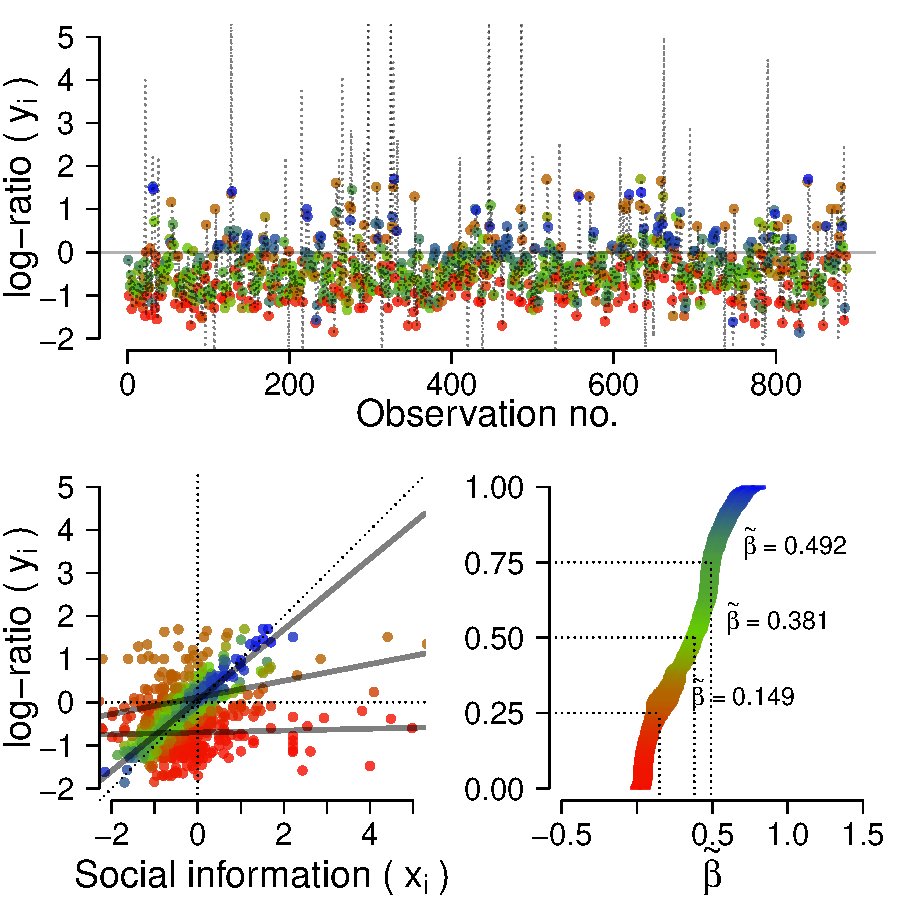
\includegraphics[width=1\linewidth]{h10971.pdf}
		\caption{\footnotesize Historical thread with $d=1097$ and $v=1$}
		\label{fig: h d=1097, v=1}
	\end{subfigure}
	\begin{subfigure}[t]{.44\linewidth}
		\centering
		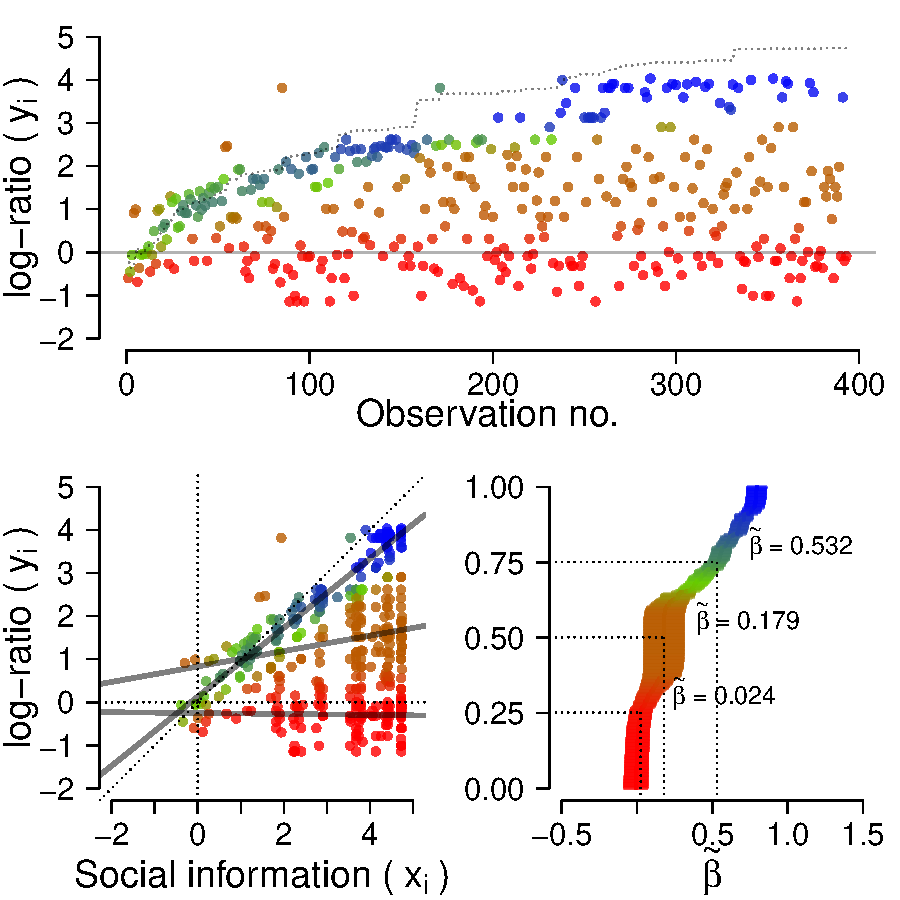
\includegraphics[width=1\linewidth]{m10979.pdf}
		\caption{\footnotesize Manipulated thread with $d=1097$ and $v=9$}
		\label{fig: m d=1097, v=9}
	\end{subfigure}
	\begin{subfigure}[t]{.1\linewidth}
		\centering
		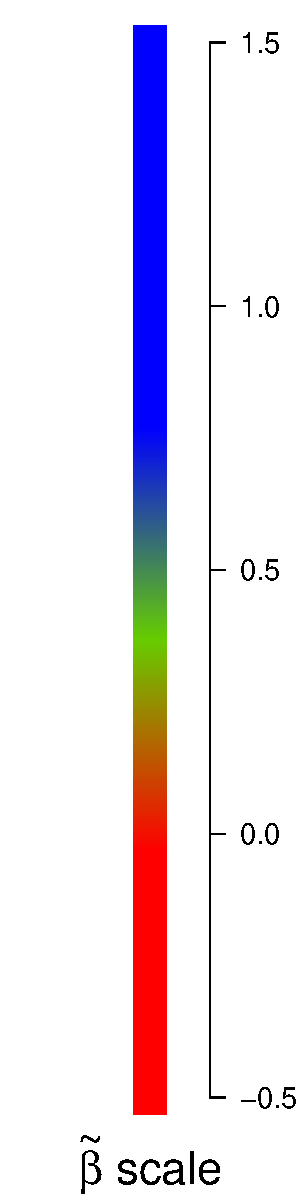
\includegraphics[width=1\linewidth]{betascale.pdf}
	\end{subfigure}
	\caption{The left hand side shows three plots of a historical thread with $d=1097$ and $v=1$, and the right hand side shows three plots of a manipulated thread with $d=1097$ and $v=9$. Top plots shows the log-ratio estimates over time (observation no.), with the geometric mean of the social information shown by a dotted line. Bottom left plots show the log-ratio of the estimates as a function of the log-ratio of the social information, indicating how differently participants use their social information. Bottom right plots show the cumulative distribution of individual $\tilde{\beta}$'s with 95\% intervals derived from the fitted models and added interquartile values of $\tilde{\beta}$.}
	\label{fig: social influence}
\end{figure*}

Contrasting timelines in Figures \ref{fig: h d=1097, v=1} and \ref{fig: m d=1097, v=9} clearly reveals different dynamics in terms of manipulation or not. In general, our experiments show distinct distributions of overlapping groups in each thread, and in the case of manipulation suggest a substantial split (or polarization) between enthusiastic persuadables versus skeptic unchangeables/contrarians. Note that the interpretation of the groups is only valid to some degree. Given a participant has a personal estimate much in line with the social information available, this participant will be seen as persuadable or as a compromiser, when in fact this is only partially true. Likewise, the group of unchangeables may consist of some few participants, whos estimate is an expression of their credulity rather than of their own belief. In general, however, the groups and their frequencies are remarkable stable across threads, which suggests that people indeed can be categorized by these proximate categories. In the supplementary material we compare our results with the results in \citet{jayles2017social} by applying our model to their data. ...

\subsubsection*{A Closer Look: A Historical Thread}
Figure \ref{fig: h d=1097, v=1} shows results for a historical thread with a rather difficult task and only a little social information available. Estimates are split among unchangeables (red), compromisers (green) and persuadables (blue) throughout the thread. Participants are prone to use whatever information is given, indicating a group of persuadables with very high $\tilde{\beta}$ values (blue). The group of unchangeables/contrarians is also quite significant, indicating that despite the difficulty, participants still weight their own opinion to a large extend. The interquartiles in the bottom right show that $\approx25\%$ are unchangeables/contrarians, where as $\approx15\%$ can be interpreted as persuadables.

%\subsubsection*{Historical thread: 403 dots and 3 views}
%\begin{figure}[htbp]
%	\centering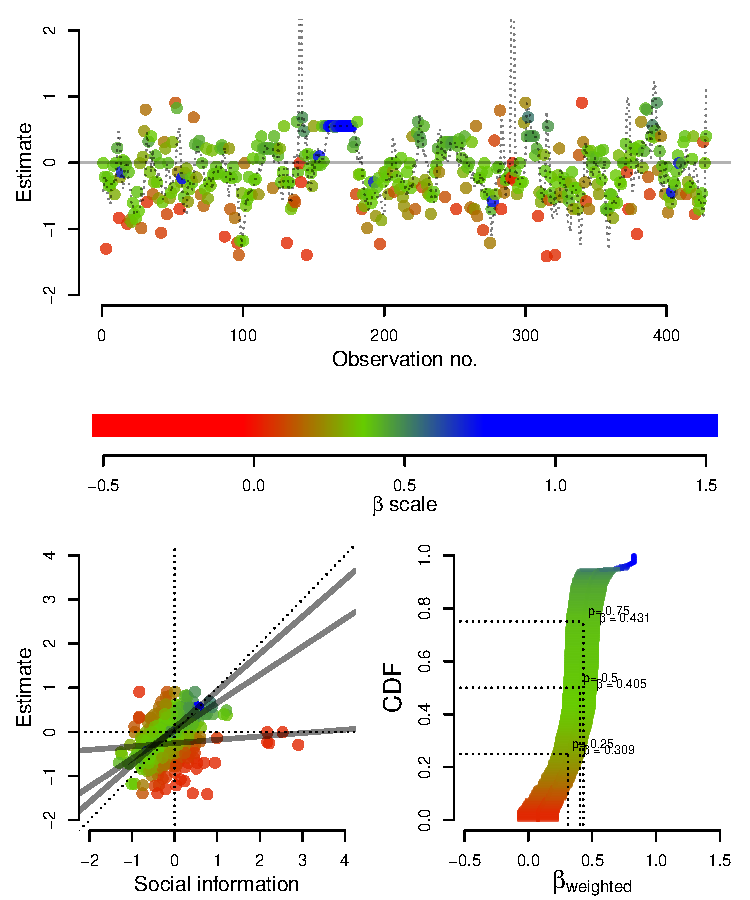
\includegraphics[width=.5\textwidth]{../plots/h4033.pdf}
%	\caption{Historical thread from the AMT experiments with 403 dots and 3 views, implying a semi-difficult %task with some social information available.}\label{fig: thread h 403 3}
%\end{figure}

%Compared to the results in Figure (\ref{fig: thread h 1097 1}), the task in this thread is also semi-difficult. With more social information given, the middle group of Compromisers (green) is larger and unchangeables/Contrarians (red) is rather small, which is also the case for the persuadables (blue). Evidently a small group of herders is present (streak of blue estimates). Compare to Figure (\ref{fig: thread h 1097 1}) it appears that with more social information participants are more prone to compromise between their own opinion and the information available.

\subsubsection*{A Closer Look: A Manipulated thread}
Figure \ref{fig: m d=1097, v=9} in contrast shows the results for a manipulated thread, where the same three groups are clearly visible, but the evolutionary trend is completely different compared to the historical thread. An interesting phenomenon is clearly displayed in the evolution of the thread. Initially the manipulation is not as pronounced, thus most participants are compromisers (green), especially due to the large amount of social information present ($v=9$). However, as the thread evolves (around 80-100 estimates in), the group splits into a small group of persuadables (blue) that drive the manipulation, and a large group of unchangeables/contrarians responding skeptically to the information presented with some participants being "suspicious" compromisers (red-brown) with lower values $\tilde{\beta}\approx 0.18$. This group clearly adopts some information, but to a much lower degree than in Figure (\ref{fig: h d=1097, v=1}). Note that the majority of green compromisers is more or less gone after 80-100 estimates, indicating that continued manipulation of a thread may lead to increased polarisation into groups of persuadables and doubtful unchangeables and/or contrarians. This split is also visible as a prototypical kink in the $\tilde{\beta}$-distribution around the 65\% quantile in the bottom right of Fig.\ref{fig: m d=1097, v=9}.

\textcolor{red}{
Here it would be nice to show an aggregated result across threads from our GMM framework. Could we for instance show in a graph of the $\tilde{\beta}$ interquartiles (25\%, 50\%, 75\%) as a function of $d$ and $v$ for manupulated/unmanipulated threads?
}

\section*{Discussion}
Sed ut perspiciatis unde omnis iste natus error sit voluptatem accusantium doloremque laudantium, totam rem aperiam, eaque ipsa quae ab illo inventore veritatis et quasi architecto beatae vitae dicta sunt explicabo. Nemo enim ipsam voluptatem quia voluptas sit aspernatur aut odit aut fugit, sed quia consequuntur magni dolores eos qui ratione voluptatem sequi nesciunt. Neque porro quisquam est, qui dolorem ipsum quia dolor sit amet, consectetur, adipisci velit, sed quia non numquam eius modi tempora incidunt ut labore et dolore magnam aliquam quaerat voluptatem. Ut enim ad minima veniam, quis nostrum exercitationem ullam corporis suscipit laboriosam, nisi ut aliquid ex ea commodi consequatur? Quis autem vel eum iure reprehenderit qui in ea voluptate velit esse quam nihil molestiae consequatur, vel illum qui dolorem eum fugiat quo voluptas nulla pariatur?

At vero eos et accusamus et iusto odio dignissimos ducimus qui blanditiis praesentium voluptatum deleniti atque corrupti quos dolores et quas molestias excepturi sint occaecati cupiditate non provident, similique sunt in culpa qui officia deserunt mollitia animi, id est laborum et dolorum fuga. Et harum quidem rerum facilis est et expedita distinctio. Nam libero tempore, cum soluta nobis est eligendi optio cumque nihil impedit quo minus id quod maxime placeat facere possimus, omnis voluptas assumenda est, omnis dolor repellendus. Temporibus autem quibusdam et aut officiis debitis aut rerum necessitatibus saepe eveniet ut et voluptates repudiandae sint et molestiae non recusandae. Itaque earum rerum hic tenetur a sapiente delectus, ut aut reiciendis voluptatibus maiores alias consequatur aut perferendis doloribus asperiores repellat.

Ad mei lucilius quaestio, virtute percipit qualisque ea his. Errem saepe delicatissimi sed ex, putent meliore maiestatis an vis. Per duis graece legimus id. At eam animal urbanitas temporibus, est ei movet definitiones, nobis blandit pertinax te his. Tritani percipit definitionem te qui, ridens maiorum patrioque pro in. Ea nec impedit apeirian facilisis, causae aliquam oporteat eam ex, ex eam ferri dolore ancillae.

Per et noster impetus. Ut nam perpetua moderatius, per forensibus theophrastus ex, ipsum definiebas sea cu. Duo id eripuit abhorreant consequuntur, nec cu audire constituto. Vim congue albucius ut. Ne pri adhuc quodsi dignissim. Ei doming dicunt pericula nec, nam ea tempor oportere temporibus, mei accusata percipitur ne.

Eu sale albucius nam, usu labores conceptam an, eam te alterum nusquam voluptatum. Usu id justo temporibus, vim an aliquip atomorum. Ne has etiam viderer noluisse, has eripuit fastidii torquatos ne. Cibo tollit euripidis pro ei.

Augue zril constituto quo ex, et omittam pertinax percipitur quo, malorum liberavisse an sit. Ius partem argumentum interpretaris at, pro mucius similique efficiantur id, mea in inani definitiones. Pro eu ubique voluptua, ut mundi viris percipitur nec. Quidam volumus lobortis mei eu, vel nominati sententiae at. Eum ut causae laoreet fastidii, tale interesset vituperatoribus has in, nemore scripserit eum te. Atomorum expetendis sadipscing cu mel, vim populo adipisci ad, an duo probo partem. Mea in tantas tritani maluisset, apeirian deseruisse mediocritatem vim ad.

In dolore diceret cum, duis vidisse albucius an his, aliquip sanctus noluisse vix et. Ad iudico persius vel, ad partem feugiat sed. Ei pri utroque necessitatibus, an sit alia minimum. His libris electram ut, nam primis timeam ut. Ei eam alia veri habemus, in dicta ocurreret accommodare vim, ei quo diam oportere abhorreant. Mel oportere conceptam ea, no doming hendrerit vel.

%The differences in the results of our dot-experiments and our experiment with an even stouter ox show that item attributes indeed matter. Estimating dots on a screen may or may not require as much expertise as estimating the stoutness of cattle, but the observed differences in the levels of herd behavior at least indicate that participants use different strategies when estimating different things. What does not differ, however, is a systematic underestimation bias of large numbers and a rapid improvement in individual as well as in collective accuracy when the number of visible preceding estimates is increased. 

%This means that the social information contained in a thread in fact helps people to calibrate their own decision-making process, even if the information may be wrong. Concerns about gullibility and correlation of judgment errors may thus be less of an evil compared to the positive effects of seeing honest opinions from other people in a thread.

%One possible reason for frequent herd behavior in the ox-threads is that participants are much more uncertain about their ability to estimate cattle weight compared to their ability to estimate dots on a screen. A high degree of uncertainty - or even an acceptance of cluelessness - may prompt participants to copy previous estimates rather than to make independent estimates by themselves \cite{navajas2018diversity}. 



\matmethods{\subsection*{Experimental design and data collection} We recruited participants from AMT to make a total of 10.808 magnitude estimations in various threads containing either an image of a certain number of dots ($d \in \{55,148,403,1097\}$) or an image of an ox ($d=1233$). After providing informed consent, participants waited in a ‘waiting room’ until the ‘choice room’ became available. When entering the choice room participants could see an image $d$ together with $v \in \{0,1,3,9\}$ previous estimates. After making an estimate, participants were thanked and paid a participation fee of \$0.10 and bonus of \$1 if their estimate was within 10\% of the true number. The average time used was less than two minutes, see SI Appendix for screenshots and detailed descriptions of the experimental design and setup.
\subsection*{Analysis of thread medians}
For observed medians $M_{dv}, d\in \{55,148,403,1097\}, v \in \{0,1,3,9\}$ the log ratios $y_{dv} = \log (M_{dv}/d)$ were modeled using a linear normal model. For a given thread, $\log{d}$ was used as a quantitative variable whereas $v$ was used as a categorical factor. Hence,  
%\begin{align}
$
	y_{dv} %= \alpha+\beta_d\sqrt{d}+\beta_0\mathbf{1}(v=0)+\beta_1\mathbf{1}(v=1)+\beta_3\mathbf{1}(v=3)+\beta_9\mathbf{1}(v=9) \\
	= \alpha+\beta_d\log{d} * \sum_{l\in\{0,1,3,9\}}\beta_l\mathbf{1}(v=l)+\varepsilon_{dv}, \label{eq: median model}
$
%\end{align}
where $*$ denotes interaction between $d$ and $v$ in the model, and $\mathbf{1}(\cdot)$ denotes the indicator function
\begin{align*}
\mathbf{1}(v=l) = \begin{cases}
								1 &\text{if } v=l \\
								0 &\text{otherwise}.
							\end{cases}
\end{align*}
The goodness of fit was assessed by analyzing the residuals $\varepsilon_{dv} \sim \mathcal{N}(0,\sigma^2)$.
\subsection*{Analysis of social influence}
As in the analysis of thread medians, individual estimates were transformed as the log-ratio, relative to the true number of dots. Thus, the modeled response variable based on $n$ observations $e_1,\dots,e_n$ from a thread with $d$ dots was $y_i = \log(e_i/d), i=1,\dots,n$. The threads were modeled individually, thus the only explanatory variable included was the social information available. However, in the experiments the participants were given either $v=1, 3$ or 9 previous estimates. Following the idea of \citep{jayles2017social} the geometric mean of these estimates was used as a measure of the social information available. As with the observed estimates, the social information was transformed as the log-ratio relative to the true number of dots $d$. If we let $z_{i,\{1,\dots,v\}}$ denote the $v$ estimates available for the $i$'th participant, then for the un-manipulated threads 
%\begin{align*}
$
	z^h_{i, \{1,\dots,v\}} = \{e_{i-1},\dots,e_{i-v}\}
$
%\end{align*}
and for the manipulated threads
$
%\begin{align*}
	z^m_{i, \{1,\dots,v\}} = \{e^*_{(1)},\dots,e^*_{(v)} | e^*_j=e_j, j<i\},
%\end{align*}
$
where $e^*_{(1)}\geq e^*_{(2)}\geq\dots\geq e^*_{(v)}\geq e^*_{(l)}, v<l\leq j<i$ denote the (decreasingly) ordered estimates $e^*_j$ among $e_1,\dots,e_j$. The superscripts $h,m$ refer to the type of information available, either historical ($h$) or manipulated ($m$). Hence, the historical information are the preceding $v$ estimates, whereas the manipulated information are the $v$ largest estimates among all preceding estimates. The quantified social information then becomes
$
%\begin{align*}
	x_i^h = \left(\prod_{l=1}^v e_{i-l} \right), \;
	x_i^m = \left(\prod_{l=1}^v e_{(j_l)} \right).
%\end{align*}
$
However, contrary to \citep{jayles2017social}, the actual estimates were available to the participants, hence in this context $x_i^{h,m}$ becomes a proxy for the available social information. %For the results using the data from \citep{jayles2017social}, in addition to the analysis using only social information as explanatory variable, another model was used where the participants estimates before social information was presented, $e_i^0, i=1,\dots,n$ was also included in it's transformed version $y^0_i, i=1,\dots,n$ to validate the interpretation of the models without this effect. As such, the two models used were
%\begin{align}
%	\begin{array}{l}
%		\mu_i = \alpha+\beta_\text{info} x_i\\
%		\mu_i = \alpha+\beta_\text{info} x_i+\beta_\text{pre}y_i^0,
%	\end{array} \quad, i=1,\dots,n  \label{eq: mean models}
%\end{align}
As such, the model used was
\begin{align}
	\mu_i = \alpha+\beta_\text{info} x_i \quad, i=1,\dots,n  \label{eq: mean models}
\end{align}
where $x_i$ is the social information available %and $y_i^0$ is the pre-information estimate of 
for observation $i$.

To cope with heavy tails present in the data, a Gaussian Mixture Model (GMM) was used to model the effects of social influence. Given $k$ states, the model fits $k$ independent Gaussian distributions with parameters $\mu_j, \sigma^2_j, j=1,\dots,k$ along with weights $\delta_{ij}, i=1,\dots, n, j=1,\dots ,k$ for each state. Note that the weight of each state is intrinsic to each of the $n$ observations. Thus, every observation is modeled as a weighted sum of (independent) Gaussian distributions, which is itself a Gaussian distribution with parameters
\begin{align}
\begin{array}{l}
	\mu_{w,i} = \sum_{j=1}^k \delta_{ij} \mu_j \\
	\sigma^2_{w,i} = \left(\sum_{j=1}^k \delta_{ij} \sigma_j\right)^2
\end{array}
\quad, i=1,\dots,n \label{eq: weighted Gaussian parameters}
\end{align}
where $\mu_{w,i}$ and $\sigma^2_{w,i}$ refer to the weighted parameter estimates for observation $i$. Applying eq. (\ref{eq: weighted Gaussian parameters}) to eq. (\ref{eq: mean models}), the effect of social information thus becomes a weighted sum of $\beta$ estimates
\begin{align}
	\beta_{w,i} = \sum_{j=1}^k \delta_{ij} \beta_{\text{info},j}, \quad i=1,\dots, n, j=1,\dots, k. \label{eq: weighted beta}
\end{align}
It should be emphasized that the weighted $\beta_{w,i}$ is unique for each observation due to the weights $\delta_{ij}$, contrary to a standard regression model where all observations are assumed to adhere to the same $\beta$ effect. For the GMM this can be interpreted as each participant is modeled as a weighted average of $k$ strategies. Hence, the personal strategy is unique, due to $\delta_{ij}$, but weighted among $k$ general axes. 
The goodness of fit for the GMM was assessed by calculating residuals
\begin{align}
 	\hat{\varepsilon}_i = \frac{y_i - \hat{\mu}_{w,i}}{\hat{\sigma}^2_{w,i}} = \begin{cases}
																							& (y_i - \hat{\alpha}-\hat{\beta}_{w,i}x_i)/\hat{\sigma}^2_{w,i} \\
																							& (y_i - \hat{\alpha}-\hat{\beta}^{\text{info}}_{w,i}x_i-\hat{\beta}^{\text{pre}}_{w,i}y^0_i)/\hat{\sigma}^2_{w,i}
																					\end{cases} \label{eq: GMM residuals}
\end{align}
and assessing the empirical distribution of $\hat{\varepsilon}_i, i=1,\dots,n$ against a standard $\mathcal{N}(0,1)$ distribution.
\subsection*{Information Criteria}
To choose a number of states $k$, each thread was fitted with 2, 3 and 4 states and the Bayesian Information Criteria (BIC) was evaluated to settle on the final $k$ states. The BIC was used rather than the more usual Akaikes Information Criteria (AIC), since the BIC penalized the number of parameters more heavily. The aim was to settle with a decent model fit, with fewer parameters to avoid overfitting. Using objective criteria to choose a number of states/clusters is often prone to simply let this number increase (ref: Tibshirani, Elements of Statistical Learning section 14.3.11) and as such the AIC yielded much larger $k$ values ($k \gg 4$).  Hence, the BIC was chosen to simplify the models more so than the AIC. 
 In our case AIC: $6k-2\ln(L)$ or BIC: $3k\ln(n)-2\ln(L)$ (note that both criteria are scaled with $3k$ parameters for $k$ states), to pick a suitable number of states. Here BIC penalizes the number of parameters weighted by the ($\log$) number of states as $3k$, corresponding to $(\delta_i,\mu_i,\sigma^2_i)$ for each state, whereas AIC only penalizes by a factor 2. 
 \subsection*{Model diagnostics}
In order to evaluate a model fit, we calculate residuals. Here we exploit the fact that a sum of (independent) gaussian components is again a gaussian. Each observation $y_l$ has an associated weighting of each state. These weights are positive and sum to 1 and can thus be interpreted as probabilities. That is, given $k$ states, the model fits $k$ gaussians with mean and variance $\hat{\mu}_i, \hat{\sigma}_i^2, i=1,\dots, k$. For the $l$'th observation, we let $\hat{\delta}_{il}$ denote the assigned probability of this observation belonging to state $i$. Note that the number of states is fixed when fitting a model, hence it does not represent a true number, but merely an assigned number of states. However, given this particular number of states, the model optimizes the fit as of which state the given observation should belong to.
Hence, for each observation $y_l$, we can calculate the residuals first by substracting the weighted mean using $\hat{\delta}_{il}, i=1,\dots,k$. By scaling with the weighted variance analogously, we obtain centered and scaled residuals that should correspond to a standard normal $\mathcal{N}(0,1)$. So we obtain the following residuals (we use the subscript $l$ on the parameters to emphasize the possible dependency on expanatory variables associated with observation $l$)
$$
  \hat{\epsilon}_l = \frac{y_l-\sum_{i=1}^k\hat{\delta}_{il}\hat{\mu}_{il} }{\sum_{i=1}^k\hat{\delta}_{il} \hat{\sigma}_{il}}\sim\mathcal{N}(0,1)\quad l=1,\dots,N
$$
}
\showmatmethods{} % Display the Materials and Methods section

\acknow{The experiments were implemented by Robin Engelhardt and Mikkel Birkegaard Andersen. Server infrastructure and devops was handled by Mikkel Birkegaard Andersen. The authors wish to thank Philipp Chapkovski for help with the cascade design, Rasmus Rendsvig for modeling discussions, Ulrik Nash and Peter Norman Sørensen for their comments on an earlier draft of this paper, and bertrand Jayles and Guy Theraulaz for sharing their data with us. This research was approved by the Institutional Review Board at the University of Copenhagen and included informed consent by all participants in the study. The authors gratefully acknowledge the support provided by The Carlsberg Foundation under grant number CF 15-0212.}
\showacknow{} % Display the acknowledgments section


% Bibliography
\bibliography{wamot}


\end{document}